\documentclass[10pt,a4paper]{amsart}
\usepackage[margin=19mm]{geometry}
\usepackage{amsmath,amssymb,mathtools}
\usepackage[scr=rsfs,cal=euler]{mathalfa}
\usepackage{xfrac}
\usepackage[unicode,hidelinks,bookmarks=false]{hyperref}
\newcommand{\ie}{i.e.\ }
\newcommand{\cf}{cf.\ }
\newcommand{\resp}{respectively\ }
\newcommand{\Subsection}{\subsection}
\providecommand{\nobreakdash}{\nobreak\hbox{-}}
\setlength{\emergencystretch}{2em}
\multlinegap0pt
\usepackage{tikz}
\usepackage{xcolor}
\usepackage{float}
\usepackage{amssymb}
\usepackage{mathtools}
\newtheorem{lemma}{Lemma}
\newtheorem{example}{Example}
\usepackage{cleveref}
\crefname{lemma}{Lemma}{Lemmas}
\crefname{example}{Example}{Examples}
\def\bfd{{\mathbf{d}}}
\def\bfr{{\mathbf{r}}}
\newcommand{\geqt}{\succeq_{\text{T}}}
\title{Varieties of Chain Complexes and Mixed Dimer Covers}
\author{Portia X. Anderson, Esther Banaian, Melanie J. Ferreri, Nicholas Mayers, Shiyun Wang, Alexander N. Wilson}
\date{Source: arXiv:2609.00202v1 (CC BY 4.0)}
\begin{document}
\maketitle

\noindent\emph{Source and licence.} Varieties of Chain Complexes and Mixed Dimer Covers. Version arXiv:2609.00202v1 (CC BY 4.0), distributed by arXiv under the Creative Commons Attribution 4.0 International licence, http://creativecommons.org/licenses/by/4.0/, as recorded in the arXiv licence metadata for this exact version and shown on the abstract page https://arxiv.org/abs/2609.00202v1. Full licence notice: \texttt{licenses/arxiv-2609.00202-CC-BY-4.0.txt}.\par\smallskip

\noindent\textit{Editorial scope.} Counted unit: the article's lemma lem:moving\_up (source0.tex lines 880--882). The article's complete original proof of it is delivered with it (source0.tex lines 884--968, one \texttt{proof} environment of 85 lines). No mathematics is written, repaired or re-derived: the statement and the proof are the article's own lines, in the article's own notation, and no retained line is substituted or re-flowed.  Retained uncounted as the source-local context the proof needs: lines 482--492; lines 872--878; lines 970--1038.  Nothing was omitted from any retained span, so the package carries no omission record.  No retained line contains a citation, so the wrapper carries no bibliography and no bibliography entry.  The retained lines contain the article's own diagram code, which the wrapper typesets with the standard tikz packages; no image file is delivered and the package declares no asset dependency.  Editorial formatting only, in addition: an AMS \texttt{amsart} preamble that restates the article's own declarations and macros used by the retained lines, namely the environments \texttt{lemma}, \texttt{example} on separate counters, together with the standard packages those lines need.  The retained environments print in this document as Lemma 1, Example 1 in order of appearance, whereas the article prints the same items with the numbering of its own full document.  The complete native source of the article as distributed in the arXiv e-print for this exact version is bundled unchanged as \texttt{sources/209002/source0.tex}.
\begin{lemma}\label{lem:VsHsDs}
If $D \in \mathcal{D}_{\mathbf{d}}$ for $\mathbf{d}\in\mathbb{Z}_{\ge 0}^n$, then the edge multiplicities in $D$ satisfy  
\begin{equation*}
 h_1(D) + v_1(D) = d_1, \qquad h_{n-1}(D) + v_n(D) = d_n. \label{}
\end{equation*}
and for all $1 \leq i \leq n-2$,
\begin{equation*}
 h_i(D) + h_{i+1}(D) + v_{i+1}(D) = d_{i+1}
\end{equation*}
Moreover, every collection of nonnegative integers $\{h_i\}_{1 \leq i \leq n-1} \cup \{v_i\}_{1 \leq i \leq n}$ satisfying these equations determines an element  $D \in \mathcal{D}_{\mathbf{d}}$. 
\end{lemma}

In this section, we provide a second bijection $\Phi$ between mixed dimer covers and rank tuples that better preserves the poset structure of each.  Let $\Phi(D)$ be the tuple $\Phi(D)=(r_1(D),\ldots,r_{n-1}(D))$ where \begin{align}
    r_i(D)=\begin{cases}
        h_i(D) & \text{for}~i~\text{even, and}\\
        \min(v_i(D),v_{i+1}(D)) & \text{for}~i~\text{odd.}
    \end{cases}.\label{eq:def_of_Phi}
\end{align}
Note that the tuple $\Phi(D)$ indeed satisfies the necessary inequalities for membership in $\mathcal{R}_\bfd$: $r_{i}+r_{i+1}\leq d_{i+1}$ for all $1\leq i\leq n-2$ and $r_i\leq m_i = \min(d_{i},d_{i+1})$ for all $2\leq i\leq n-1$.  

\begin{example}\label{ex:moving_up}
Below we show the process described in \Cref{lem:moving_up} for a particular $\bfd$-dimer cover
with $\bfd=(4,5,7,3)$. At each stage, the most recently twisted cell is
shaded. Note that because $v_4(D_1)<v_3(D_1)$, we have no twist in the subsequent step,
so $D_2=D_1$.

\[\begin{array}{ccc}
    \raisebox{.34in}{$D=$}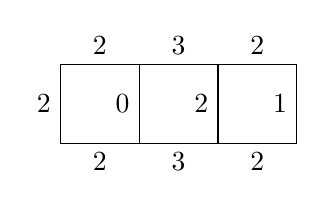
\begin{tikzpicture}[scale=.5]
      \draw (0,0) rectangle (2,2);
      \draw (2,0) rectangle (4,2);
      \draw (4,0) rectangle (6,2);
      \node at (1,2) [above] {$2$};
      \node at (3,2) [above] {$3$};
      \node at (5,2) [above] {$2$};
      \node at (1,0) [below] {$2$};
      \node at (3,0) [below] {$3$};
      \node at (5,0) [below] {$2$};
      \node at (0,1) [left]  {$2$};
      \node at (2,1) [left] {$0$};
      \node at (4,1) [left] {$2$};
      \node at (6,1) [left] {$1$};
    \end{tikzpicture} &  \raisebox{.34in}{$\longleftrightarrow$} & \raisebox{.34in}{$\Phi(D)=(0,3,1)$}\\
        \raisebox{.34in}{$D_1=$}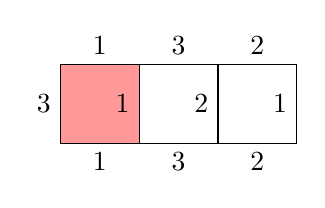
\begin{tikzpicture}[scale=.5]
      \draw[fill=red!40!white] (0,0) rectangle (2,2);
      \draw (2,0) rectangle (4,2);
      \draw (4,0) rectangle (6,2);
      \node at (1,2) [above] {$1$};
      \node at (3,2) [above] {$3$};
      \node at (5,2) [above] {$2$};
      \node at (1,0) [below] {$1$};
      \node at (3,0) [below] {$3$};
      \node at (5,0) [below] {$2$};
      \node at (0,1) [left]  {$3$};
      \node at (2,1) [left] {$1$};
      \node at (4,1) [left] {$2$};
      \node at (6,1) [left] {$1$};
    \end{tikzpicture} & & \\
        \raisebox{.34in}{$D_2=$}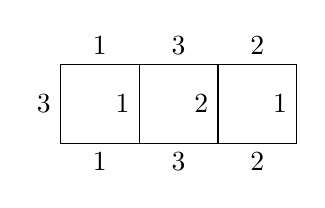
\begin{tikzpicture}[scale=.5]
      \draw (0,0) rectangle (2,2);
      \draw (2,0) rectangle (4,2);
      \draw (4,0) rectangle (6,2);
      \node at (1,2) [above] {$1$};
      \node at (3,2) [above] {$3$};
      \node at (5,2) [above] {$2$};
      \node at (1,0) [below] {$1$};
      \node at (3,0) [below] {$3$};
      \node at (5,0) [below] {$2$};
      \node at (0,1) [left]  {$3$};
      \node at (2,1) [left] {$1$};
      \node at (4,1) [left] {$2$};
      \node at (6,1) [left] {$1$};
    \end{tikzpicture} &  & \\
        \raisebox{.34in}{$D'=$}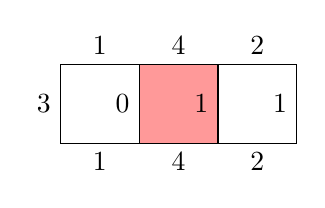
\begin{tikzpicture}[scale=.5]
      \draw (0,0) rectangle (2,2);
      \draw[fill=red!40!white] (2,0) rectangle (4,2);
      \draw (4,0) rectangle (6,2);
      \node at (1,2) [above] {$1$};
      \node at (3,2) [above] {$4$};
      \node at (5,2) [above] {$2$};
      \node at (1,0) [below] {$1$};
      \node at (3,0) [below] {$4$};
      \node at (5,0) [below] {$2$};
      \node at (0,1) [left]  {$3$};
      \node at (2,1) [left] {$0$};
      \node at (4,1) [left] {$1$};
      \node at (6,1) [left] {$1$};
    \end{tikzpicture} &  \raisebox{.34in}{$\longleftrightarrow$} & \raisebox{.34in}{$\Phi(D')=(0,4,1)$}\\
\end{array}\]
\end{example}

\begin{lemma}\label{lem:moving_up}
    Let $\mathbf{d}=(d_1,\hdots,d_n)$ and $\mathbf{r}=(r_1,r_2,\ldots,r_{n-1})\in \mathcal{R}_{\mathbf{d}}$. If \[\mathbf{r}'=(r_1,r_2,\ldots,r_{i-1},r_i+1,r_{i+1},\ldots,r_{n-1})\in \mathcal{R}_{\mathbf{d}}\] and $\mathbf{r}=\Phi(D)$ for some $D\in \mathcal{D}_{\mathbf{d}}$, then there exists $D'\in\mathcal{D}_{\mathbf{d}}$ such that $\Phi(D')=\mathbf{r}'$ and $D'\geqt D$.
\end{lemma}

\begin{proof}
We are concerned with the piece of the $\bfd$-dimer cover $D$ consisting of tiles $i-1$, $i$, and $i+1$
from the left, which we illustrate in the following diagram.

\[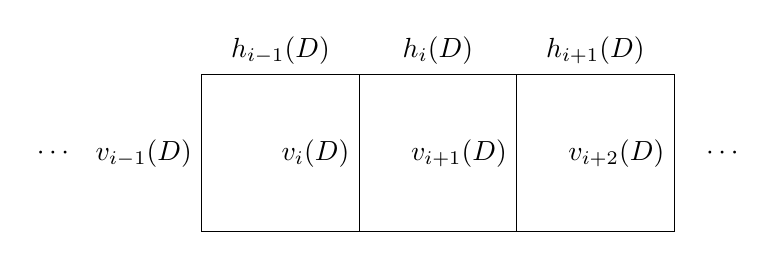
\begin{tikzpicture}[scale=1]
  \draw (0,0) rectangle (2,2);
  \draw (2,0) rectangle (4,2);
  \draw (4,0) rectangle (6,2);

  \node at (1,2) [above] {$h_{i-1}(D)$};
  \node at (3,2) [above] {$h_i(D)$};
  \node at (5,2) [above] {$h_{i+1}(D)$};
  \node at (0,1) [left]  {$v_{i-1}(D)$};
  \node at (2,1) [left] {$v_i(D)$};
  \node at (4,1) [left] {$v_{i+1}(D)$};
  \node at (6,1) [left] {$v_{i+2}(D)$};
  
  \node at (-1.5,1) [left] {$\cdots$};
  \node at (7,1) [left] {$\cdots$};
\end{tikzpicture}\]

Since $\mathbf{r}' \in \mathcal{R}_{\mathbf{d}}$, we must have strict inequalities $r_i < m_i$, $r_{i-1} + r_i < d_i$ and $r_i + r_{i+1} < d_{i+1}$.

In order to analyze further, we split into two cases based on the parity of $i$. Throughout the proof, set $h_0(D) = h_{n-1}(D) = 0$ and $v_0(D) = v_{n}(D) =0$.
First assume that $i$ is odd. Then $r_{i-1} = h_{i-1}(D)$ and $r_{i+1} = h_{i+1}(D)$ for $D$ such that $\Phi(D) = \mathbf{r}$. In this case, either
\begin{enumerate}
    \item[(i)] $\min(v_i(D),v_{i+1}(D))=v_i(D)$, in which case we consider
    \begin{align*}
        r_{i-1}'+r_i'=r_{i-1}+(r_i+1)&\le d_i,\\
        \intertext{and by definition of $\Phi$ and Lemma \ref{lem:VsHsDs}, we replace the left and right sides respectively to obtain}
        h_{i-1}(D)+v_i(D)+1 &\le h_{i-1}(D)+v_i(D)+h_i(D),
    \end{align*}
    so that $h_i(D) > 0$, or
    \item[(ii)] $\min(v_i(D),v_{i+1}(D))=v_{i+1}(D)$, in which case we consider
    \[r_i'+r_{i+1}'\leq d_{i+1}\]
    and similarly find that $h_i(D)>0$.
\end{enumerate}

Thus, in either case $h_i(D)$ is positive and one can apply a horizontal twist at tile $i$ of $D$ resulting in the desired $\mathbf{d}$-dimer cover $D'$.

Next assume that $i$ is even. In this case, we need to form two intermediate $\bfd$-dimer covers, $D_1$ and $D_2$ on our way to $D'$. The reader may wish to follow along using \Cref{ex:moving_up}. We form $D_1$ as follows. If $v_{i-1}(D)<v_i(D)$, then we simply let $D_1=D$ and note that $v_i(D_1)=v_i(D)>0$. If instead $v_{i-1}(D)\geq v_i(D)$, then we note that \begin{align*}
    h_{i-1}(D)&=d_i-(h_i(D)+v_i(D)) & \text{by Lemma \ref{lem:VsHsDs}}\\
    &=d_i-(r_{i}+r_{i-1}) & \text{by \Cref{eq:def_of_Phi}}\\
    &\geq1 & \text{by $\bfr'\in R_\bfd$.}
\end{align*}
This allows us to apply a horizontal twist at tile $i-1$ of $D$, yielding $D_1\in\mathcal{D}_\bfd$. We make the following observations about $D_1$ that hold in both cases: \begin{enumerate}
    \item[(a1)] $D_1\geqt D$,
    \item[(b1)] $v_i(D_1)>0$, and
    \item[(c1)] $v_i(D_1)-v_i(D)=\delta_{v_{i-1}(D)\geq v_i(D)}$ and similarly for $v_{i-1}$.
\end{enumerate}
where for a statement $S$, we have that $\delta_S$
is the quantity $1$ when $S$ is true and the quantity
$0$ when $S$ is false.

Now, we form $D_2$ from $D_1$ similarly. If $v_{i+2}(D_1)<v_{i+1}(D_1)$, then we simply let $D_2=D_1$ and note that $v_{i+1}(D_2)=v_{i+1}(D_1)>0$. If instead $v_{i+2}(D_1)\geq v_{i+1}(D_1)$, then we note that
\begin{align*}
    h_{i+1}(D_1)=h_{i+1}(D)&=d_i-(h_i(D)+v_{i+1}(D)) & \text{by Lemma \ref{lem:VsHsDs}}\\
    &=d_i-(r_i+r_{i+1})& \text{by \Cref{eq:def_of_Phi}}\\
    &\geq 1 & \text{by $\bfr'\in R_\bfd$.}
\end{align*}
This allows us to apply a horizontal twist at tile $i+1$ of $D_1$, yielding $D_2\in\mathcal{D}_\bfd$. We make the
following observations about $D_2$ that hold in both cases:\begin{enumerate}
    \item[(a2)] $D_2\geqt D_1$,
    \item[(b2)] $v_{i+1}(D_2)>0$, and
    %\item[(c2)] $v_{i+1}(D_2)-v_{i+1}(D_1)=\delta_{v_{i+2}(D_1)\geq v_{i+1}(D_1)}=\delta_{v_{i+2}(D)\geq v_{i+1}(D)}$ and similarly for $v_{i+2}$.
\end{enumerate}

Finally, because $v_i(D_2)=v_i(D_1)>0$ and $v_{i+1}(D_2)>0$, we form a $\bfd$-dimer cover $D'$ from $D_2$ by performing a vertical twist at tile $i$. Note that by transitivity, $D'\succ_T D$.
Because we changed values only at squares $i-1$, $i$, and $i+1$, we have that $\Phi(D')$ can only differ from $\bfr=\Phi(D)$ at indices $i-1$, $i$ and $i+1$. Our final twist at tile $i$ ensures that 
\begin{align*}
    \Phi(D')_i&=h_i(D)+1=r_i+1.
\end{align*}
Now, working back through the modifications of each twist, we have that
\begin{align*}
    \Phi(D')_{i-1}&=\min(v_{i-1}(D'),v_{i}(D'))\\
    &=\min(v_{i-1}(D_2),v_i(D_2)-1)\\
    &=\min(v_{i-1}(D_1),v_i(D_1)-1)\\
    &=\min(v_{i-1}(D),v_i(D)-1)+\delta_{v_{i-1}(D)\geq v_i(D)}.
\end{align*}
If $v_{i-1}(D)\geq v_i(D)$, this resolves to $v_{i}(D)-1+1=v_{i}(D)$.
If instead $v_{i-1}(D)< v_i(D)$, this resolves to $v_{i-1}(D)$. Hence, $\Phi(D')_{i-1}=\min(v_{i-1}(D),v_i(D))=r_{i-1}$. Similarly, $\Phi(D')_{i+1}=r_{i+1}$ and $\Phi(D')=\bfr'$ as desired.

We have demonstrated the result for all values of $i$ other than $i=1$ and $i=n$. These two remaining cases are analogous and in fact simpler. \qedhere

\end{proof}

\end{document}
